\phantomsection
\chapter{Introduction}

There are many unanswered questions about the mysteries of the mind and brain. One of the major mysteries, and also one of the primary characteristics of us as humans, is Language. By Language here we do not mean the specific instances such as English, Hindi, German, etc. but rather the general ability of Language. This ability enables us to convey the most abstract ideas that our minds can create, in the form of strings of arbitrary sounds or signs, as well as to decode and receive the said information and ideas from these strings of arbitrary sounds or signs.

From this perspective, we could define Language as an information encoding system \cite{coupe2019different}, through which we encode our thoughts into strings of speech sounds or signs to communicate these thoughts to others. To reiterate, information in our mind is encoded (or in a manner - translated) into a string of speech sounds or signs, which after going through a medium is received by the recipient, who then decodes these sequence of speech sounds or signs, receiving the information to be conveyed, thus completing the process of communication \cite{shannon1948mathematical}.

\begin{figure}[h]
    \centering
    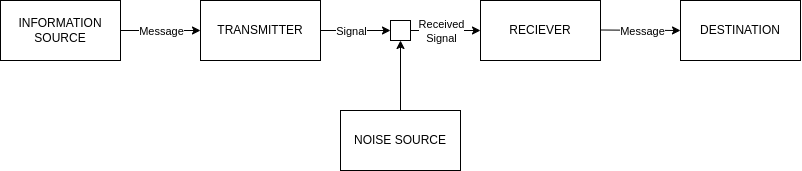
\includegraphics[width=0.96\textwidth]{images/InformationProcess.drawio.png}
    \caption{Shannon's model of the process of communication}
\end{figure}

Translation may be seen as another step added to this process. Information encoded in one language (\gls{sl}) is to be transferred into an utterance in another language (\gls{tl}). In a way, the nature of the process of translation is similar to that of the nature of Language itself, both are trying to maintain the integrity of meaning/information changing from one form to another. Well, even that is an oversimplification of the idea of translation and the phenomenon of language.

\phantomsection
\section{Translation}

 The human experience thrives on stories, ideas, and emotions, all intricately woven with the threads of language. Yet, the very beauty of language lies in its diversity, a vibrant tapestry of tongues that both connects and separates us. Language is one yet languages are many, this distinction and the necessity to bridge this gap is why we need translation \cite{ricoeur2007translation}. Translation is far from a simple act of word substitution. It's a labyrinthine journey, a constant negotiation between being faithful to the source text and the need to create a work that resonates with the target audience, while also being mindful of the socio-cultural contexts of this bilateral exchange.
 
Many theorists have presented their definition of translation focusing on various paradigms. Catford for one defines translation as ``{\itshape the replacement of textual material in one language (\gls{sl}) by equivalent textual material in another language (\gls{tl}).}", this approach draws upon a theory of language, a general linguistic theory \cite{catford1965linguistic}. In this definition, the focus is on meticulously replacing textual material in the source language with its closest counterpart in the target language. Imagine a meticulous puzzle, where each piece from the source language must find its perfect fit in the target language, ensuring accuracy in the transfer of information. This approach prioritizes faithfulness to the literal meaning of the text, relying on established linguistic theories for guidance.
 
 Nida presents a different view emphasizing the message involved in this exchange, he proposes the idea of dynamic equivalence and defines translation as - ``{\itshape the closest natural equivalent of the source-language message, first in terms of meaning and secondly in terms of style}" \cite{nida1964toward} \cite{jixing2013translation}. The aim is to create a text in the target language that resonates with the new audience in the same way the original resonated with its intended readers, by capturing not just the raw meaning of the words, but also the stylistic nuances, the emotional weight, and the cultural references embedded within the original work.

 The complexity involved in the translation process is observed, endowing it with the characteristics of both an art and a science \cite{nida1964toward} \cite{bell2016translation}.

\phantomsection
\section{Machine Translation}

Commerce and war have been a major driving force behind several technological advances, which also include translation. Translation is a necessity when it comes to the interaction and trade beyond geographical boundaries. Even though geograp-hical limitations have been somewhat overcome, bringing people closer in the vast virtual world, the problem of communication stands, and so does the necessity of translation \cite{bhattacharyya2015machine}. 

\gls{mt} was brought into serious consideration in the 1950s with the advent of modern computers. It was the first computer-based application of \gls{nlp} \cite{hutchins1992introduction}. Since then the progress of Machine Translation has not exactly been linear. The \gls{alpac} report of 1966 dealt a heavy blow to the development of Machine Translation, nearly halting more of the developments in this field \cite{poibeau20171966}. Yet the developments did not completely stop, and \gls{mt} has since come a long way. Though it has not achieved human-level accuracy \cite{rivera2022machine}, it still produces astonishing results.

\gls{mt} has seen a lot of developments in the past few decades. Providing an overview of these developments is one of the objectives of this work, especially highlighting the progress made in the last two decades, especially in the context of \gls{nmt}. Although modern machine translation approaches are mostly data-driven, there have been other approaches whose impact is still prevalent.

\gls{rbmt} and Data-Driven or Corpus-Based MT are two major approaches under which most of the techniques for Machine Translation fall \cite{bhattacharyya2015machine}. RMBT techniques were the first approach adopted; some of the techniques involved were direct approach, involving the use of bilingual dictionaries and morphological analysis to translate the source text word by word without much focus on the syntactic nuances of the SL or TL.  Transfer-based and Interlingua MT, in which the attempt is to convert the Source Text into an intermediate representation, a formal one for transfer-based techniques, and an abstract one for Interlingua, which is then converted to the Target Language Text \cite{baker2019routledge}.

The advent of the information age and the increase in both computing power and availability of large corpora lead to the development of data-driven/corpora-based MT techniques. \gls{smt} and \gls{ebmt} are the outcomes of these developments \\ \cite{baker2019routledge}. SMT learns from a massive collection of bilingual texts to translate languages. It uses a "translation model" to find the most likely translations of words and phrases, and a "language model" to ensure that the translated sentences are grammatically correct \cite{hutchins2006future}. However, EBMT works like a giant library of translated examples. When given a new text to translate, EBMT searches this library for the closest existing translations (matching). Then it identifies the relevant parts from those translations (alignment) and recombines them to fit the new text grammatically (recombination).


\phantomsection
\subsection{Neural Machine Translation}

Leveraging modern high-performance computing and massive amounts of data, has allowed a new technology for Machine Learning to take form, i.e. Artificial Neural Networks, especially Deep Neural Networks. The application of this technology in translation has given rise to a new approach - Neural Machine Translation (NMT). The work has been going on for quite a while, for example, Robert B. Allen's demonstration of the use of a feed-forward neural network to translate from English to Spanish with a vocabulary length of 31 \cite{allen1987several}.

\begin{figure}[h]
    \centering
    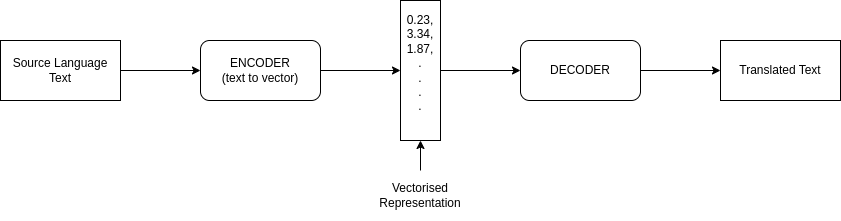
\includegraphics[width=0.96\textwidth]{images/EncoderDecoder.png}
    \caption{Encoder-Decoder Architecture}
    \label{fig:encode-decode}
\end{figure}

A major breakthrough in this approach was made in 2013-14, with the use of Convolutional Neural Networks (CNNs) and Recurrent Neural Networks (RNNs) to encode SL text into an intermediate representation, which was then decoded using an RNN-based decoder for TL \cite{kalchbrenner2013recurrent} \\ \cite{cho2014learning} \cite{sutskever2014sequence}. There were limitations to this approach, i.e., they faced difficulties when dealing with longer sentences, which was addressed with the introduction of {\itshape Attention} \cite{bahdanau2014neural}. Attention was an important component that led to the development of Large Language Models (LLMs).

Google in 2016 released a massive NMT system, which performed quite well, making NMT a go-to research area for most of the translation research since then \cite{wu2016google}. In 2017 came the paper titled "Attention is all you need" \cite{vaswani2017attention} which revolutionized Artificial Intelligence, giving rise to massive Multi-modal Large Language Models, enabling various technologies to take shape, especially language technologies. Though most of the NMT systems today are sequence-to-sequence models, they have become much more powerful and effective.

\phantomsection
\section{Legal Translation}

The importance of language in law is an indisputable fact. Just like any other form of human communication and affairs, human law cannot exist without language, but language is a complicated matter. It enables us to tell truths, lies, truths that seem like lies, and lies that seem like truth. Ambiguity in law is a fatal flaw, and ambiguity, more often than not has the potential to turn up in language use.

Legal language needs to be very particular and accurate, this presents a very peculiar problem for translators, where they not only have to focus on finding an equivalence for the message but also preserve its structure integrity in a disambiguate manner.

In modern times where numerous tasks have been handed over to machines, especially translation, and it's application for legal translation isn't too far off. The use of Machine Translation in a legal context will become prevalent, but to what extent is yet to be seen. One must be very careful with such sensitive matters as \cite{deborah2023challenges} exemplifies - 

\begin{quote}
Translation, especially in legal contexts, can carry significant consequen-ces. After all, one may never know whether the translation of the Chinese word 夷 \textit{yi} or 蛮夷 \textit{manyi} as ‘barbarians’ or ‘foreign barbarians’, as opposed to ‘foreigners’, contributed to the start of the Opium Wars (1839–1860) between China and Western countries all those years ago.
\end{quote}

As we must have all experienced, this kind of error is one of the prevalent flaws of many MT systems. Thus, the use of MT for a sensitive application such as legal translation must be done under numerous considerations.

\phantomsection
\section{Indian Penal Code}

The \gls{ipc}, while no longer in use, is an extremely important document in India's legal history, and defined India's criminal code for over one and a half centuries, until recently, when it was replaced by Bharatiya Nyaya Sanhita in December 2023. 

Drafted in 1860 by the British Raj, it aimed to be a unified code covering all major crimes \cite{devadas2016history}. It outlines various offenses, from theft and assault to murder and treason. It also established a system of punishments, including imprisonment, fines, and even the death penalty. The code aimed to be clear and concise, ensuring everyone understood what constituted a crime and its corresponding consequences.

The IPC was broadly categorized into four parts. The initial chapters (I-V) laid the groundwork, defining legal terms and establishing principles of liability. Chapters VI-XV then addressed offenses impacting the state, public order, and safety. Chapters XVI-XXII formed the core, encompassing crimes between individ-uals like theft, assault, and property damage. Finally, Chapter XXIII served as a safety net for uncategorized attempts to commit crimes \cite{devadas2016history}.

Let's look at an excerpt from IPC, Chapter VIII - Section 144:-

\begin{quote}
    \emph{\textbf{English}} \\ \textbf{Joining unlawful assembly armed with deadly weapon} — Whoever, being armed with any deadly weapon, or with anything which, used as a weapon of offense, is likely to cause death, is a member of an unlawful assembly, shall be punished with imprisonment of either description for a term which may extend to two years, or with fine, or with both.
\end{quote}

\begin{quote}
\emph{\textbf{{\hindifont हिंदी}}} \\
 \textbf{{\hindifont घातक आयुध से सज्जित होकर विधिविरुद्ध जमाव में सम्मिलित होना}} -  {\hindifont जो कोई किसी घातक आयुध से, या किसी ऐसी चीज से, जिससे आक्रामण आयुध के रुप में उपयोग कये जाने पर मृत्र्यु कारित होनी सम्भाव्य है, सज्जित होते हुए किसी विधिविरुद्ध जमाव का सदस्य होगा, वह दोनों में से किसी भांति के कारावास से, जिसकी अवधि दो वर्ष तक की हो सकेगी, या जुर्माने से या दोनों से, दण्डित किया जायेग। }
\end{quote}


\phantomsection
\section{Theoretical Framework: Dorr's Divergence}

Bonnie J. Dorr, in her paper titled "Machine Translation Divergences: A Formal Description and Proposed Solution" \cite{dorr1994machine}, talks about various issues which come up when a translation task is taken up, these issues are termed as translation divergences, these divergences are essentially cross linguistic differences which make the direct linear transfer from SL to TL impractical. She presents solutions to these divergences in her paper, which are derived from the formalization of two types of information - (1) the linguistically grounded classes upon which lexical-semantic divergences are based; and (2) the techniques by which lexical-semantic divergences are resolved. Let us take a look at some of the divergences proposed by Dorr.

\paragraph{Thematic Divergence}

Thematic Divergence involves the repositioning of the arguments with respects to a head, a change in the thematic role of the argument. This type of divergence arises only in cases in which there is a logical subject present.

\begin{quote}
English: I like Mary \\
Spanish: Maria me gusta a mi (Mary pleases me)    
\end{quote}

\paragraph{Promotional Divergence}

Promotional Divergence connotes the promotion of logical modifier into a main verb position, i.e. logical modifier becomes the syntactic head and the syntactic head becomes an internal argument.

\begin{quote}
English: John usually goes home \\
Spanish: Juan suele ir a casa (John tends to go home)
\end{quote}

\paragraph{Demotional Divergence}

Demotional Divergence is the opposite of Promotional Divergence, i.e., logical head gets associated with syntactic adjunct position and logical argument is associated with syntactic head position.

\begin{quote}
English: I like eating \\
German: Ich esse gern (I eat likingly)
\end{quote}

\paragraph{Structural Divergence}

Structural Divergence results in change of the syntactic class associated with a syntactic constituent.

\begin{quote}
English: John entered the house \\
Spanish: Juan entro en la casa (John entered the house)
\end{quote}

\paragraph{Conflational Divergence}

Conflational Divergence occurs when sense of one word in SL is described by more than one word in TL.

\begin{quote}
English: I stabbed John \\
Spanish: Yo le di punaladas a Juan (I gave knife-wounds to John)
\end{quote}

\paragraph{Categorical Divergence}

Categorical Divergence happens when part-of-speech (POS) property of a word/constituent in SL changes during translation to TL.

\begin{quote}
English: I am hungry \\
German: Ich habe hunger (I have hunger)
\end{quote}

\paragraph{Lexical Divergence}

Lexical Divergence happens when there is no exact equivalent of a word/constituent in SL in TL, thus some other word/constituent is used to express a sense which is somewhat similar to the original sense.

\begin{quote}
English: John broke into the room \\
Spanish: Juan forzo la entrada al cuarto (John forced (the) entry to the room)
\end{quote}

There are several other types of divergences as discussed by Dorr. These divergences are an important basis for judging machine translation systems.

\phantomsection
\section{Motivation for Research}

For our course in Semester IX, concerned with computational linguistics, we had to analyze the systematic divergences observed in translating short stories from Hindi to English. Though the translation was more often than not, acceptable, there was still situations where the divergences posed were severe and caused a major loss of sense in the process of translation. This may be fine in the case of non-consequential texts like a short story, but in the case of things like legal texts, contracts, and judgments, minor cases of linguistic ambiguity, let alone such major divergences have major consequences. Thus, with the aim to analyze the development and systematic performance of these tools, I took up this study. 

\phantomsection
\section{Problem Identification}

As highlighted, even though MT has come a long way, it is still far from perfect. There are still several sets of issues present. For resource-rich languages such as English, German, etc. this set of issues is small, but for languages lacking resources and also for language pairs with a wide difference between their syntactic and morphological structures, this set is still large. Issues like lexical divergence, syntactic divergence, improper cognate transfer, and artificiality are still present, and in the case of legal translation, these kinds of divergences might present serious issues. 

English is the most resource-rich language, and Hindi could be said to have the largest speaker base in India. Translation between these two languages should be relatively better, compared to a language pair such as Japanese and Santali. But how accurate would it be in terms of accuracy, and how the issues observed would create problems for translating legal text is what we wished to explore in this study, while also appreciating how far the field of Machine Translation has come.

\phantomsection
\section{Research Questions}

\begin{itemize}
    \item How has Machine Translation developed over the decades?
    \item What is the performance of modern Machine Translation tools?
\end{itemize}

\phantomsection
\section{Objectives}

\begin{itemize}
    \item To summarize the development of Machine Translation over the decades.
    \item To evaluate the effectiveness of Machine Translation tools, with a focus on legal translation.
\end{itemize}

\phantomsection
\section{Limitations}

For this study took a sample of the 511 Sections of the IPC in Hindi, and translate them into English by using two NMT tools - Google Translate and Azure Translate. After translating we analyzed the translation. We used automated metrics, as well as human evaluation. The details of the sampling, analysis, the metrics, and the tools used are discussed in detail in Chapter \ref{chap:meth}.

The metrics we used for this study are BLEU and ROUGE, both of these approaches require multiple reference translations to perform well, but in the case of this study, we have been only able to provide one reference translation. Also, only one human participant was employed to score the translations. However, these limitations do not have that great of an influence on the result of this study, as we do get a rough picture of where these translation tools stand.